\chapter{Perceptual Experiments}
\label{chap:PerceptualExperiments}

\section{Introduction}
\label{sec:PerceptualExperiments-Introduction}
	This chapter discusses two experiments to evaluate the performance of harmonic excitations systems based on those
	discussed in Chapter \ref{chap:FeatureControl}. The first experiment (Section
	\ref{sec:PerceptualExperiments-Reconstruction}) compares the abilities of different excitation methods in
	generating individual harmonics to reconstruct degraded signals. The second experiment (Section
	\ref{sec:PerceptualExperiments-SemanticControl}) uses the results discussed in Chapter \ref{chap:TimbreEvaluation}
	to inform the design of harmonic excitation effects which provide control over a particular perceptual parameter.
	In both experiments the performance of the systems under test is evaluated using both objective metrics and
	subjectively through perceptual listening tests.

\section{Reconstruction of Individual Harmonics}
\label{sec:PerceptualExperiments-Reconstruction}
	Several of the harmonic excitation systems discussed in Section \ref{sec:FeatureControl-Systems} rely on the
	generation of individual harmonics of the input signal. Ideally, when a new harmonic is added to a signal using one
	of these systems it should sound `natural'. The resulting signal should sound as though it came from a single
	source. A poorly generated harmonic may be perceived as a new sinusoid completely separate from the original input
	signal. Harmonic generation methods can be evaluated by how `naturally' they can reconstruct signals from which
	harmonics have been removed. In this section an experiment is described evaluating the performance of three
	different harmonic generation methods.

	\subsection{Harmonic Reconstruction Systems}
	\label{sec:PerceptualExperiments-Reconstruction-Systems}
		Missing harmonics can be reintroduced to a signal by generating them from the remaining information in the
		degraded signal. This can be achieved using a spectral shaping system similar to that shown in Figure
		\ref{fig:SpectralShapingSystem}. Rather than shaping the spectrum to achieve a musical effect it is used to
		reconstruct the shape of the original spectrum. The missing harmonics are generated individually with the
		amplitudes they had in the original (non-degraded) signal. In this section three methods of generating
		these individual harmonics are discussed.

		The first method of reconstructing the harmonics is based on synthesis of new sinusoids and is illustrated
		in Figure \ref{fig:Synthesise}. The STFT of the input signal is calculated and used to generate an
		amplitude envelope for the input signal's fundamental. This amplitude envelope is then used in the
		synthesis of a sinusoid at the frequency of the desired harmonic.

		\begin{figure}[h!]
			\centering
			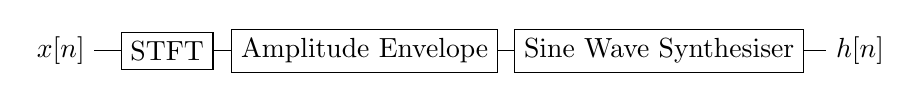
\begin{tikzpicture}
				\node (In) at (-0.1, 1) {$x[n]$};
				\node (STFT) [draw] at (1.25, 1) {STFT};
				\draw (In) -- (STFT);

				\node (Amp) [draw] at (3.76, 1) {Amplitude Envelope};
				\draw (STFT) -- (Amp);

				\node (Synth) [draw] at (7.5, 1) {Sine Wave Synthesiser};
				\draw (Amp) -- (Synth);

				\node (Out) at (10.05, 1) {$h[n]$};
				\draw (Synth) -- (Out);
			\end{tikzpicture}
			\caption{}
			\label{fig:Synthesise}
		\end{figure}

		The other two harmonic generation methods use the system illustrated in Figure \ref{fig:FilterAndShift},
		isolating the fundamental with a low pass filter and then using a frequency shifting technique to change
		the frequency to that of the desired harmonic. The two frequency shifting techniques used in this
		experiment are SSBA (Section \ref{sec:Excitation-Methods-SSBA}) and IAP (Section
		\ref{sec:Excitation-Methods-IAP}).

		\begin{figure}[h!]
			\centering
			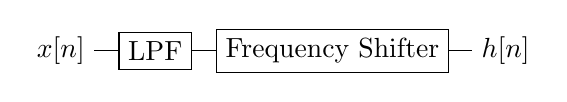
\begin{tikzpicture}
				\node (In) at (1.3, 1) {$x[n]$};
				\node (Filter) [draw] at (2.5, 1) {LPF};
				\draw (In) -- (Filter);

				\node (Exciter) [draw] at (4.75, 1) {Frequency Shifter};
				\draw (Filter) -- (Exciter);

				\node (Out) at (6.95, 1) {$h[n]$};
				\draw (Exciter) -- (Out);
			\end{tikzpicture}
			\caption{}
			\label{fig:FilterAndShift}
		\end{figure}

	\subsection{Methodology}
	\label{sec:PerceptualExperiments-Reconstruction-Methodology}
		\subsubsection*{Stimuli Generation}
			The harmonic reconstruction systems were evaluated using the same four audio signals used in
			Section \ref{sec:FeatureControl-Parameterisation} to assess audio feature parameterisation
			techniques (cello, clarinet, synthesised and piano). For each signal the third through ninth
			harmonics were removed. This was in order to cause significant degradation in the quality of the
			signal such that the difference is plainly audible to the majority of listeners. The second
			harmonic was left in the signal to pose a challenge to the SSBA and IAP methods. As mentioned in
			previously the performance of these methods depends on how well the fundamental is isolated.
			Retaining the second harmonic allows for the effect of filter order on the performance of the
			system to be assessed. Spectrograms of the cello signal before and after this process are shown in
			Figures \ref{fig:CelloSpectrogram} and \ref{fig:CelloFilteredSpectrogram}. 

			\begin{figure}[h!]
				\centering
				\captionsetup[subfigure]{oneside,margin={1cm, 0cm}}
				\subfloat[Unprocessed Signal]
				{
					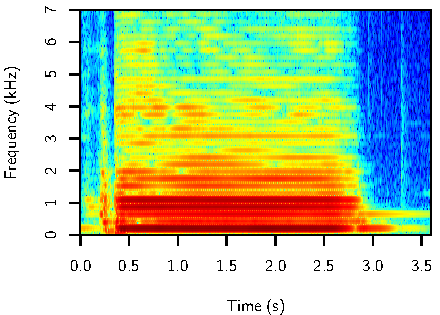
\includegraphics{chapter7/Images/CelloSpectrogram.pdf}
					\label{fig:CelloSpectrogram}
				}
				\quad
				\subfloat[Filtered Signal]
				{
					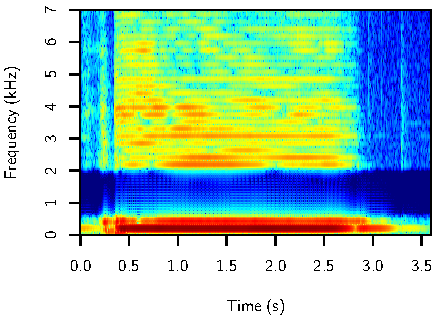
\includegraphics{chapter7/Images/CelloFilteredSpectrogram.pdf}
					\label{fig:CelloFilteredSpectrogram}
				}
				\caption{Spectrograms of the cello signal.}
				\label{fig:CelloSpectrograms}
			\end{figure}

			Test stimuli were created by reintroducing the third through ninth harmonics to the filtered
			signals using the systems described in Section
			\ref{sec:PerceptualExperiments-Reconstruction-Systems}. In order to reduce the number of variables,
			each of the unprocessed signals was analysed prior to the creation of the test stimuli. The
			fundamental frequency of each signal was measured along with the amplitudes of the third through
			ninth harmonics. This information was then used in the reconstruction of the signal mitigating any
			inaccuracies which may be introduced by calculating it in real time and allowing the `naturalness'
			of the generated harmonics to be assessed more thoroughly.

			Eleven test stimuli were created from each of the original four signals. The first two being the
			unprocessed signal and the filtered signal. The remaining nine were reconstructions of the original
			signal from the filtered signal. Each signal was reconstructed three times using each system, using
			different parameters each time. For the synthesis method the window length of the STFT was changed,
			taking values of 50, 100 and 500 samples. As the window length increases the frequency resolution
			of the spectrum increases allowing for more accurate calculation of the amplitude of the
			fundamental.  Longer window length however will decrease the temporal resolution of the system,
			smoothing the extracted amplitude envelope. Care must be taken to not increase the STFT window
			length such that this smoothing starts to reduce the accuracy of the extracted amplitude envelope.
			For the SSBA and IAP methods a different order FIR filter was used to isolate the fundamental
			frequency. The filters used were windowed sinc filters with orders of 50, 100 and 500 and using the
			Blackman window to maximise stopband attenuation \citep{schlichtharle2011digital}. As the filter
			order increases the fundamental is better isolated reducing the level of any intermodulation
			components.

		\subsubsection*{Objective Evaluation}
			An approximation of the perceptual difference between the stimuli and the relevant audio signal is
			measured using the R\sub{nonlin} metric proposed by \citet{tan2004predicting}. As discussed in
			Section \ref{sec:Excitation-Analysis-Metrics} this is a metric which uses psychoacoustic models of
			the human hearing system to judge the perceived level of distortion in a signal. It is calculated
			by comparing the degraded signal against the non-degraded signal, returning a value between 0 and
			1. 1 denoting a signal which is indistinguishable from the original and lower values describing
			signals with a higher level of perceivable distortion.

		\subsubsection*{Subjective Evaluation}
			The performance of the reconstruction systems was evaluated subjectively using series of multiple
			stimulus listening tests using the MUSHRA methodology \citep{mushra2014}. Each tests is split into
			two phases, a training phase and an evaluation phase. In the training phase participants are
			presented with an interface (Figure \ref{fig:MushraTraining}) which allows them to audition every
			one of the stimuli. The stimuli which are the unprocessed versions of the original signals are
			identified as the reference stimuli. Participants are asked to listen to each of the stimuli in
			comparison with the relevant reference in order to learn the range of degradation across stimuli.
			Once they have auditioned every stimulus they are able to proceed to the evaluation phase.

			\begin{figure}[h!]
				\centering
				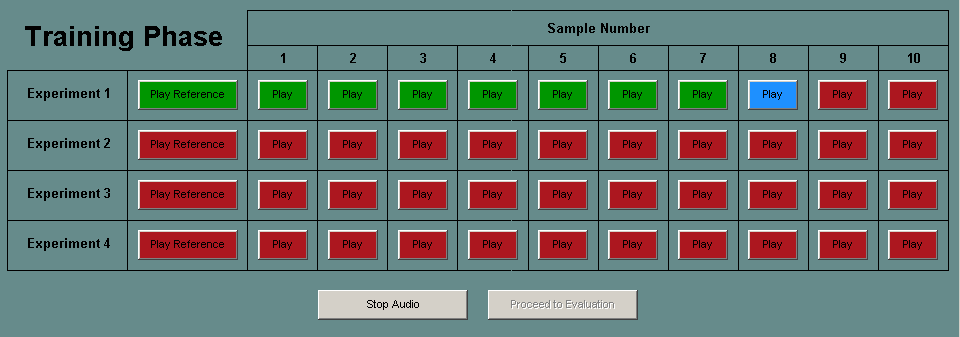
\includegraphics[width=0.8\textwidth]{chapter7/Images/MushraTraining.png}
				\caption{The training phase interface.}
				\label{fig:MushraTraining}
			\end{figure}

			During the evaluation phase participants are presented with all stimuli created from the same
			signal at once. They were asked to grade how well each of the stimuli recreate the reference
			stimuli (the unprocessed signal) on a scale from 0 to 100. The scale is shown in Figure
			\ref{fig:MushraScale} and the full interface in Figure \ref{fig:MushraEvaluation}.

			\begin{figure}[h!]
				\centering
				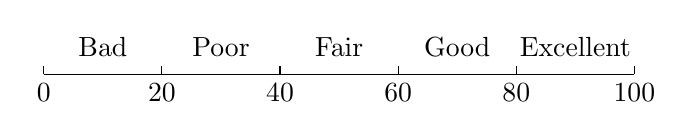
\begin{tikzpicture}
					\draw(0, 0) -- (7.5, 0);

					\foreach \x/\xvalue in {0/0, 1.5/20, 3/40, 4.5/60, 6/80, 7.5/100}
						\draw (\x, 0pt) -- (\x, 3pt)
						(\x, 0pt) node[below] {\xvalue};

					\foreach \x/\xtext in {0.75/Bad, 2.25/Poor, 3.75/Fair, 5.25/Good, 6.75/Excellent}
						\draw (\x, 3pt) node[above] {\xtext};
				\end{tikzpicture}
				\caption{The grading scale used in the evaluation phase.}
				\label{fig:MushraScale}
			\end{figure}

			Among the stimuli to be graded were a hidden reference and anchor. These are included in order to
			assess the performance of test participants. The hidden reference is a repetition of the reference
			signal and as such should be given a grade of 100 as there is no difference between it and the
			reference. The anchor is the filtered signal and should be graded worse than the all the other
			stimuli as no attempt has been made to reconstruct the signal. If a participant does not grade the
			hidden reference and anchor in this way their results may not be reliable.

			\begin{figure}[h!]
				\centering
				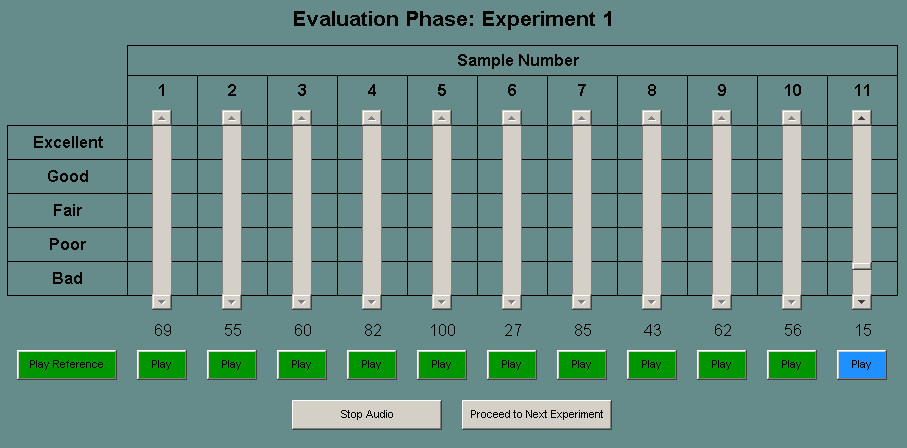
\includegraphics[width=0.8\textwidth]{chapter7/Images/MushraEvaluation.png}
				\caption{The evaluation phase interface.}
				\label{fig:MushraEvaluation}
			\end{figure}

			This evaluation phase is repeated for each of the original audio signals. The order in which the
			evaluation phases for each signal were presented to participants was randomised along with the
			order in which the stimuli appear in the interface in order to mitigate any effect the order in
			which stimuli are heard may have on the results.

			Listening tests were undertaken using circumaural headphones in a quiet listening environment. In
			total eight participants took part in the listening tests, all of whom reported no know hearing
			problems. On average participants spent 5.14 minutes in the training phase ($\sigma$ = 1.85) and
			3.36 minutes on each of the four evaluation phases ($\sigma$ = 20.6).

	\subsection{Results}
	\label{sec:PerceptualExperiments-Reconstruction-Results}
		In the results figures presented in this section the eleven stimuli created from each test signal are
		numerated 1 to 11 as follows:

		\begin{tabular}{>{\bfseries}rl}
			1. & The reference stimulus. \tabularnewline
			2. & Stimulus reconstructed using the synthesis method with an STFT window length of 50
			     samples. \tabularnewline
			3. & Stimulus reconstructed using the synthesis method with an STFT window length of 100
			     samples. \tabularnewline
			4. & Stimulus reconstructed using the synthesis method with an STFT window length of 500
			     samples. \tabularnewline
			5. & Stimulus reconstructed using the SSBA method using a 50\super{th} order filter. \tabularnewline
			6. & Stimulus reconstructed using the SSBA method using a 100\super{th} order filter.
			     \tabularnewline
			7. & Stimulus reconstructed using the SSBA method using a 500\super{th} order filter.
			     \tabularnewline
			8. & Stimulus reconstructed using the IAP method using a 50\super{th} order filter. \tabularnewline
			9. & Stimulus reconstructed using the IAP method using a 100\super{th} order filter. \tabularnewline
			10. & Stimulus reconstructed using the IAP method using a 500\super{th} order filter.
			     \tabularnewline
			11. & Stimulus with third through ninth harmonics removed (anchor).
		\end{tabular}

		The R\sub{nonlin} results for each of the stimuli are presented in Figure \ref{fig:SMCRNonlin}. The values
		have been normalised to the range 0 to 100 for purposes of comparison with the grading scale used in the
		listening test. Note that for the piano signal three of the reconstructed stimuli have R\sub{nonlin} score
		lower than that of the anchor. This is due to the piano signal having a damped fundamental.  Reconstructing
		the higher order harmonics using information in the fundamental produces lower quality harmonics as the
		structure of the fundamental does not reflect that of the other harmonics in the signal. In lieu of this,
		test participants who grade any of the reconstructed piano stimuli less than the piano anchor will not be
		deemed unreliable.
		
		Two of the eight participants who took part in the listening tests failed to grade the hidden reference
		correctly causing their results have been discarded. The mean grades given by the remaining six
		participants are shown in Figure \ref{fig:SMCRNonlin} with error bars illustrating 95\% confidence
		intervals. The Pearson correlation ($r$) between these mean grades and the R\sub{nonlin} scores for the
		stimuli are shown in Table \ref{tab:SMCCorrelations}.

		\begin{figure}[h!]
			\centering
			\captionsetup[subfigure]{oneside,margin={1cm, 0cm}}
			\subfloat[Cello Stimuli]
			{
				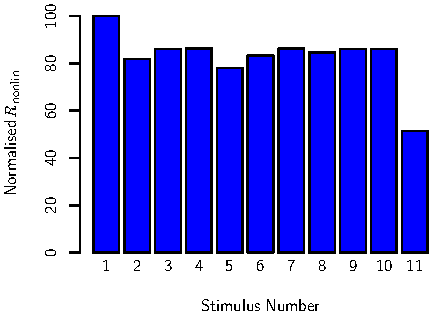
\includegraphics{chapter7/Images/CelloRNonlin.pdf}
				\label{fig:CelloRNonlin}
			}
			\quad
			\subfloat[Clarinet Stimuli]
			{
				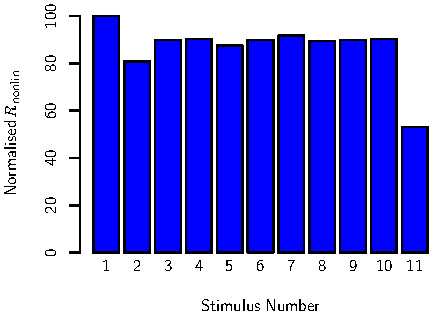
\includegraphics{chapter7/Images/ClarinetRNonlin.pdf}
				\label{fig:ClarinetRNonlin}
			}

			\subfloat[Synthesised Stimuli]
			{
				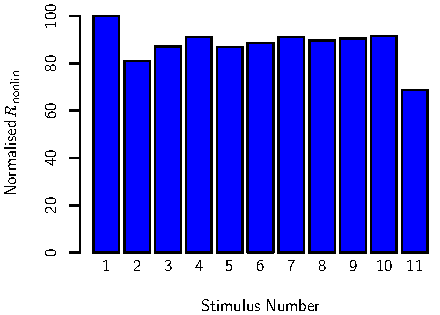
\includegraphics{chapter7/Images/SynthRNonlin.pdf}
				\label{fig:SynthRNonlin}
			}
			\quad
			\subfloat[Piano Stimuli]
			{
				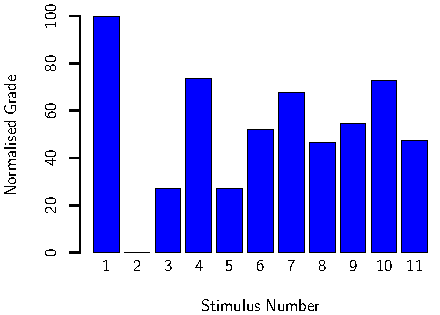
\includegraphics{chapter7/Images/PianoRNonlin.pdf}
				\label{fig:PianoRNonlin}
			}
			\caption{R\sub{nonlin} values for each of the stimuli.}
			\label{fig:SMCRNonlin}
		\end{figure}

		\begin{figure}[h!]
			\centering
			\captionsetup[subfigure]{oneside,margin={1cm, 0cm}}
			\subfloat[Cello Stumuli]
			{
				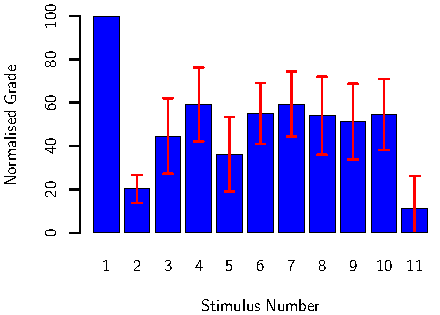
\includegraphics{chapter7/Images/CelloResults.pdf}
				\label{fig:CelloResults}
			}
			\quad
			\subfloat[Clarinet Stimuli]
			{
				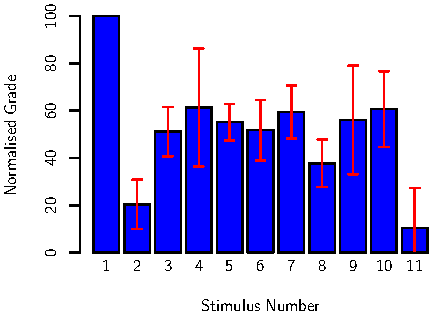
\includegraphics{chapter7/Images/ClarinetResults.pdf}
				\label{fig:ClarinetResults}
			}

			\subfloat[Synthesised Stimuli]
			{
				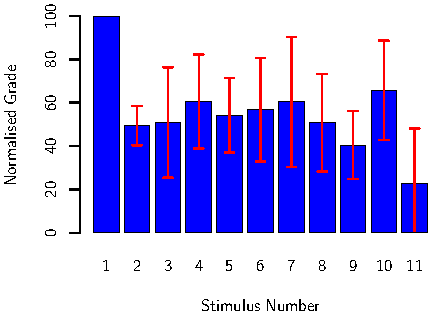
\includegraphics{chapter7/Images/SynthResults.pdf}
				\label{fig:SynthResults}
			}
			\quad
			\subfloat[Piano Stimuli]
			{
				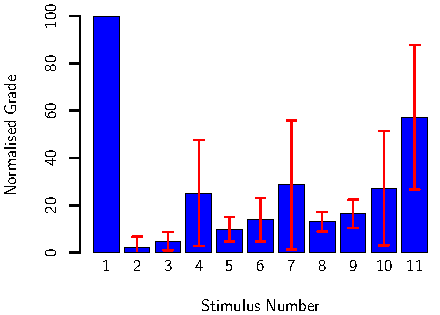
\includegraphics{chapter7/Images/PianoResults.pdf}
				\label{fig:PianoResults}
			}
			\caption{Mean grades and confidence intervals for each of the stimuli.}
			\label{fig:SMCResults}
		\end{figure}

		\begin{table}[h!]
			\centering
			\begin{tabular}{|c|c|c|}
	\hline
	\bf{Signal} & $\boldsymbol{r}$ & $\boldsymbol{p}$ \tabularnewline
	\hline
	\hline
	Cello & 0.83 & 0.001 \tabularnewline
	\hline
	Clarinet & 0.82 & 0.002 \tabularnewline
	\hline
	Synthesised & 0.85 & 0.001 \tabularnewline
	\hline
	Piano & 0.73 & 0.011 \tabularnewline
	\hline
\end{tabular}

			\caption{Correlations between the R\sub{nonlin} values and the mean grades.}
			\label{tab:SMCCorrelations}
		\end{table}

	\subsection{Discussion}
	\label{sec:PerceptualExperiments-Reconstruction-Discussion}
%		\begin{figure}[h!]
%			\centering
%			\captionsetup[subfigure]{oneside,margin={1cm, 0cm}}
%			\subfloat[Synthesis with an STFT window length of 50 samples.]
%			{
%				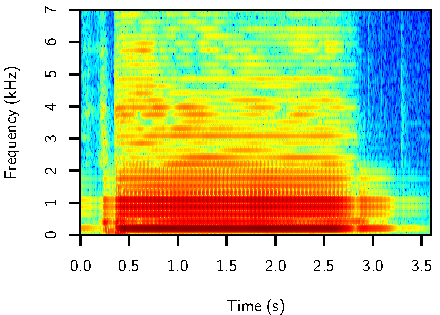
\includegraphics{chapter7/Images/CelloSynthesisSpectrogram.pdf}
%				\label{fig:CelloSynthesisSpectrogram}
%			}
%			\quad
%			\subfloat[SSBA with a 50\super{th} order filter.]
%			{
%				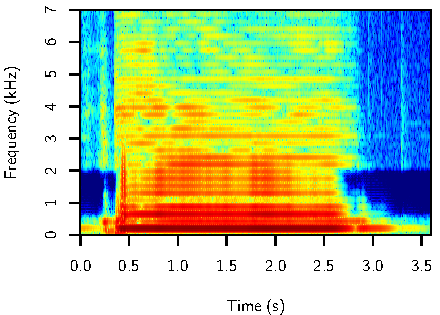
\includegraphics{chapter7/Images/CelloSSBASpectrogram.pdf}
%				\label{fig:CelloSSBASpectrogram}
%			}
%			
%			\subfloat[IAP with a 50\super{th} order filter.]
%			{
%				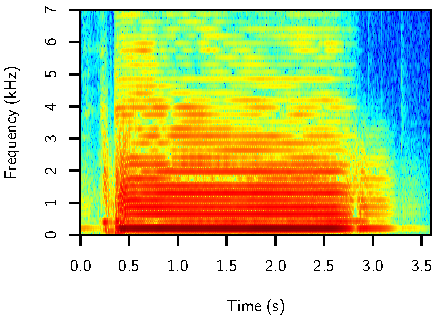
\includegraphics{chapter7/Images/CelloIAPSpectrogram.pdf}
%				\label{fig:CelloIAPSpectrogram}
%			}
%			\caption{Spectrograms of the cello stimulus reconstructed using three different methods.}
%			\label{fig:ReconstructedCelloSpectrograms}
%		\end{figure}
%
%		\begin{figure}[h!]
%			\centering
%			\captionsetup[subfigure]{oneside,margin={1cm, 0cm}}
%			\subfloat[Temporal Envelopes]
%			{
%				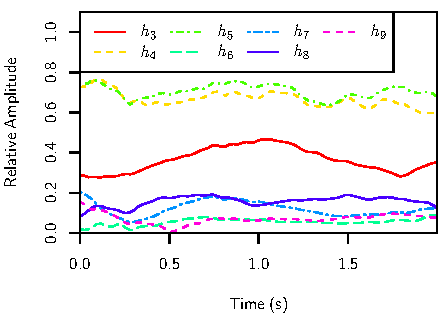
\includegraphics{chapter7/Images/CelloHarmonicAmplitudes.pdf}
%				\label{fig:CelloAmps}
%			}
%			\quad
%			\subfloat[Amplitude Distributions]
%			{
%				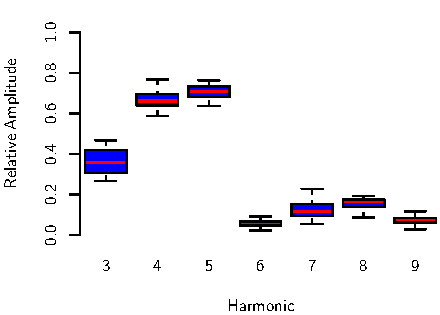
\includegraphics{chapter7/Images/CelloHarmonicAmplitudeBoxs.pdf}
%				\label{fig:CelloBoxs}
%			}
%			\caption{The amplitude ratios between the third through ninth harmonics 
%				 and the fundamental in the cello signal.}
%			\label{fig:CelloHarmonics}
%		\end{figure}
%
%		\begin{figure}[h!]
%			\centering
%			\captionsetup[subfigure]{oneside,margin={1cm, 0cm}}
%			\subfloat[Temporal Envelopes]
%			{
%				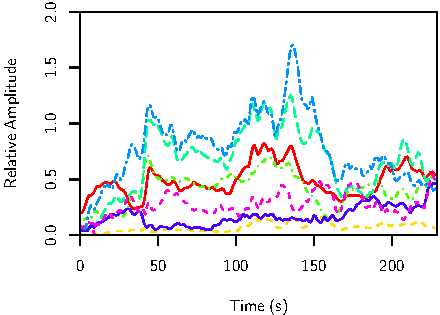
\includegraphics{chapter7/Images/ClarinetHarmonicAmplitudes.pdf}
%				\label{fig:ClarinetAmps}
%			}
%			\quad
%			\subfloat[Amplitude Distributions]
%			{
%				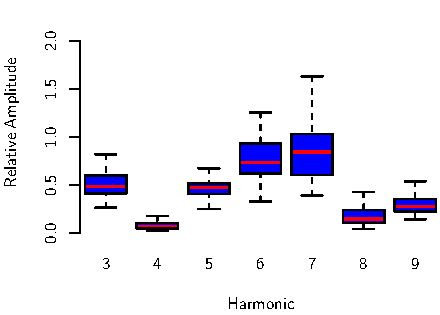
\includegraphics{chapter7/Images/ClarinetHarmonicAmplitudeBoxs.pdf}
%				\label{fig:ClarinetBoxs}
%			}
%			\caption{The amplitude ratios between the third through ninth harmonics 
%				 and the fundamental in the clarinet signal.}
%			\label{fig:ClarinetHarmonics}
%		\end{figure}
%
%		\begin{figure}[h!]
%			\centering
%			\captionsetup[subfigure]{oneside,margin={1cm, 0cm}}
%			\subfloat[Temporal Envelopes]
%			{
%				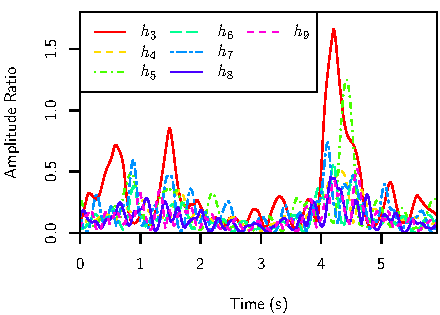
\includegraphics{chapter7/Images/SynthHarmonicAmplitudes.pdf}
%				\label{fig:SynthAmps}
%			}
%			\quad
%			\subfloat[Amplitude Distributions]
%			{
%				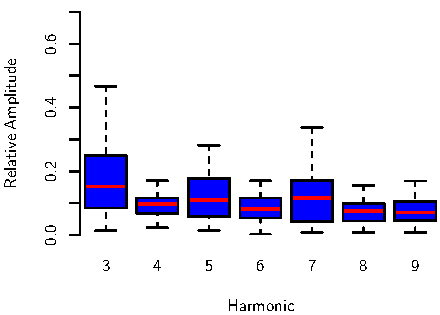
\includegraphics{chapter7/Images/SynthHarmonicAmplitudeBoxs.pdf}
%				\label{fig:SynthBoxs}
%			}
%			\caption{The amplitude ratios between the third through ninth harmonics 
%				 and the fundamental in the synthesised signal.}
%			\label{fig:SynthHarmonics}
%		\end{figure}
%
%		\begin{figure}[h!]
%			\centering
%			\captionsetup[subfigure]{oneside,margin={1cm, 0cm}}
%			\subfloat[Temporal Envelopes]
%			{
%				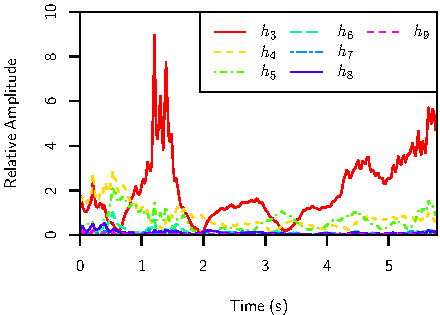
\includegraphics{chapter7/Images/PianoHarmonicAmplitudes.pdf}
%				\label{fig:PianoAmps}
%			}
%			\quad
%			\subfloat[Amplitude Distributions]
%			{
%				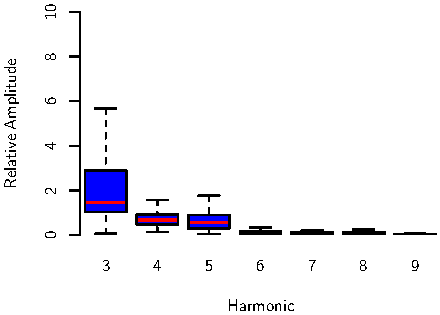
\includegraphics{chapter7/Images/PianoHarmonicAmplitudeBoxs.pdf}
%				\label{fig:PianoBoxs}
%			}
%			\caption{The amplitude ratios between the third through ninth harmonics 
%				 and the fundamental in the piano signal.}
%			\label{fig:PianoHarmonics}
%		\end{figure}
%
		The results of the listening test show that the effects of STFT window length and filter order are as
		expected. Across the majority of the stimuli there is an increase in the perceived quality of the
		reconstruction as the STFT window length / filter order is increased. The R\sub{nonlin} measurements
		confirm that as these parameters are increased the resulting reconstructed signal is objectively more
		similar to the original signal. For each of the original signals the reconstruction with a window length /
		filter order of 500 receive similar grades, it is in the lower setting of these parameters that differences
		between the methods become noticeable.

		For each of the acoustic signals (cello, clarinet and piano) the reconstruction with the synthesis method
		and an STFT window length of 50 samples was given the lowest mean grade by test participants. This is most
		likely because of the poor spectral resolution achieved when using such a short analysis window. The SSBA
		and IAP techniques produce better reconstructions of these signals at lower filter orders and require less
		computational power. The results for the synthesised sample do not exhibit this pattern, with the IAP
		reconstructions being given lower grades than the other methods for lower filter orders. However, examining
		the R\sub{nonlin} measures it is seen that the IAP reconstructions of this signal are objectively more
		similar to the original signal than those reconstructed with the synthesis method. This is possibly
		explained by the fact that the synthesised signal is the easiest to reconstruct. It is a purely harmonic
		signal with no energy at inharmonic frequencies. This makes it easy to isolate the fundamental and produce
		harmonics with less intermodulation components. As all the reconstructions of the synthesised signal are
		similar to each other it is more difficult for test participants to decide where to grade them on the
		scale.  Where there is more variability between the stimuli, as for the acoustic signals, it becomes easier
		for test participants to grade stimuli on the scale as they will need to be spread over a wider larger
		range.

		All the systems evaluated in this section use the amplitude envelope of the fundamental to inform the
		amplitude envelopes of the generated harmonics. This assumes that the amplitude envelopes of the harmonics
		in a signal have a simple relationship with that of the fundamental. A linear relationship is assumed by
		both the IAP and synthesis based systems while the SSBA system assumes a polynomial relationship which is
		dependant on the order of the harmonic being generated. These assumptions introduce inaccuracies in the
		reconstruction of signals in which the amplitudes of the harmonics do not obey these relationships. Better
		results might be achieved by using one of the higher order harmonics in the generation of new harmonics,
		rather than the fundamental. For the synthesis method, measuring the amplitude of this harmonic and for the
		SSBA and IAP methods filtering this harmonic out and shifting its frequency to the desired value. For the
		cello sample, for instance, it may be better to use the fundamental in the generation of the third harmonic
		but the second harmonic in the generation of the other harmonics as the amplitude envelopes of those
		combinations are better matched as seen in Figure \ref{fig:CelloSpectrogram}. Building a system like this
		however, requires knowledge of which harmonics in the input signal will be the best choice for
		reconstructing a given harmonic. This will be different depending on the source of the signal and is not
		calculable from a degraded input signal. Furthermore, the SSBA and IAP techniques are only able apply
		frequency shifts at integer multiples of the frequency of the input signal. In order to generate all orders
		of harmonic using these techniques the fundamental must be used as the input to the frequency shifter.
		
		The degree of inaccuracy introduced can be estimated by examining the relationships of the harmonics'
		amplitudes in the unprocessed test signals. As the systems rely on the fundamental's amplitude envelope
		this relationship will be measured as the ratio between the amplitude of each harmonic and that of the
		fundamental $\left(\frac{h_{n}}{h_{1}}\right)$. Depending on the source of the sound, and playing method if
		it was produced by an acoustic instrument, the relationships between the harmonics' amplitudes may be
		different in the attack, sustain and release portions of the signal. Figures \ref{fig:AttackAmplitudes} to
		\ref{fig:ReleaseAmplitudes} show the amplitude ratios between the third through ninth harmonics of the test
		signals and their fundamentals.

		\note
		{
			If you have a gander at Figure \ref{fig:AttackAmplitudes} you can see that they have 8 colours and
			some lines what wiggle about and shit (Stasis, 2017).
		}

		\begin{figure}[h!]
			\centering
			\captionsetup[subfigure]{oneside,margin={1cm, 0cm}}
			\subfloat[Cello Signal]
			{
				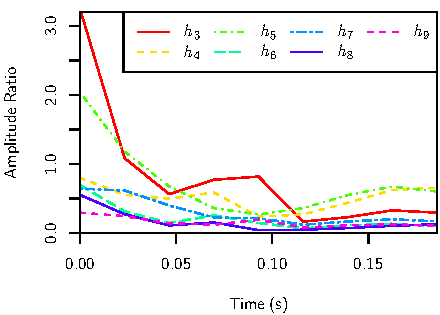
\includegraphics{chapter7/Images/CelloAttackAmplitudes.pdf}
				\label{fig:CelloAttack}
			}
			\quad
			\subfloat[Synthesised Signal]
			{
				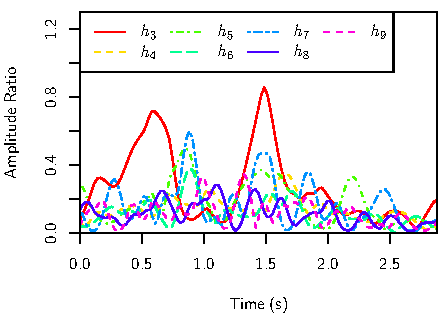
\includegraphics{chapter7/Images/SynthAttackAmplitudes.pdf}
				\label{fig:SynthAttack}
			}

			\subfloat[Piano Signal]
			{
				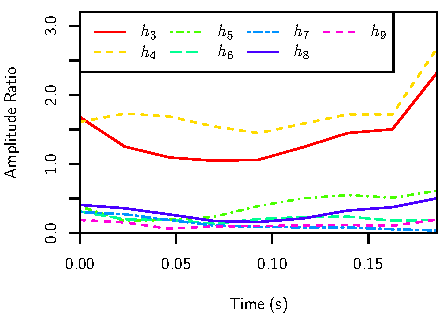
\includegraphics{chapter7/Images/PianoAttackAmplitudes.pdf}
				\label{fig:PianoAttack}
			}
			\caption{Amplitude ratios between the harmonics and fundamental in the attack and decay
				 portions of the test signals.}
			\label{fig:AttackAmplitudes}
		\end{figure}

		Figure \ref{fig:AttackAmplitudes} shows the amplitude ratios between the harmonics and fundamental for the
		attack and decay portions of the test signals. The clarinet signal is not included as its attack portion is
		too fast to apply spectral analysis. The cello signal (Figure \ref{fig:CelloAttack}) has a fast attack
		followed by a slower decay in which the amplitudes of the higher harmonics decay quicker than that of the
		fundamental. The synthesised signal (Figure \ref{fig:SynthAttack}) has a slow attack and release in which
		the in which the amplitudes increase and decrease more rapidly than that of the fundamental. This signal
		also exhibits individual amplitude modulation of each of the harmonics. In the attack and decay portions of
		the piano signal (Figure \ref{fig:PianoAttack}) the amplitude ratios remain mostly consistent.

		\begin{figure}[h!]
			\centering
			\captionsetup[subfigure]{oneside,margin={1cm, 0cm}}
			\subfloat[Cello Signal]
			{
				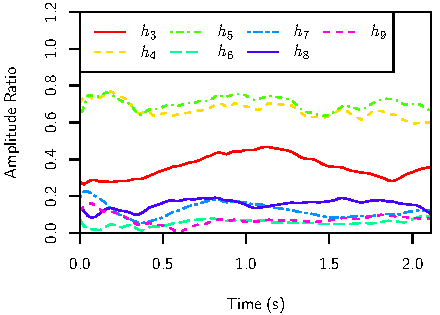
\includegraphics{chapter7/Images/CelloSustainAmplitudes.pdf}
				\label{fig:CelloSustain}
			}
			\quad
			\subfloat[Clarinet Signal]
			{
				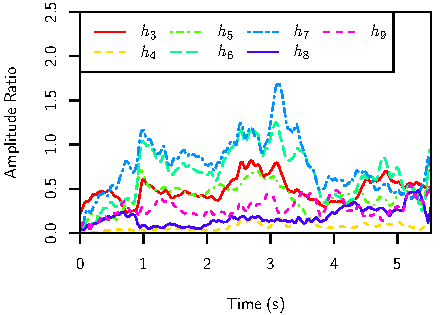
\includegraphics{chapter7/Images/ClarinetSustainAmplitudes.pdf}
				\label{fig:ClarinetSustain}
			}

			\subfloat[Synthesised Signal]
			{
				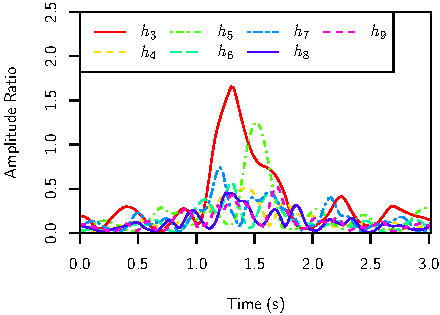
\includegraphics{chapter7/Images/SynthSustainAmplitudes.pdf}
				\label{fig:SynthSustain}
			}
			\quad
			\subfloat[Piano Signal]
			{
				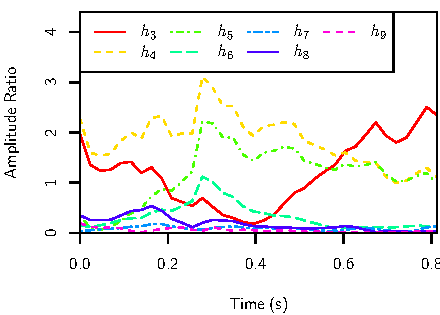
\includegraphics{chapter7/Images/PianoSustainAmplitudes.pdf}
				\label{fig:PianoSustain}
			}
			\caption{Amplitude ratios between the harmonics and fundamental in the sustain
				 portions of the test signals.}
			\label{fig:SustainAmplitudes}
		\end{figure}

		Figure \ref{fig:SustainAmplitudes} shows the amplitude ratios between the harmonics and fundamental for the
		sustain portions of the test signals. Of the signals, the cello signal has the most consistent amplitude
		ratios in its sustain portion (Figure \ref{fig:CelloSustain}). The amplitude ratios in the sustain section
		of the synthesised signal oscillate about low levels apart from at one instance in which the amplitudes of
		the odd order harmonics exhibit high peaks. The clarinet and piano signals have more complex sustain
		sections in which the amplitudes of the individual harmonics vary greatly. In the clarinet signal (Figure
		\ref{fig:ClarinetSustain}) the harmonics amplitudes appear to change in unison with one another but
		independently from the fundamental. In the piano signal's sustain section (Figure \ref{fig:PianoSustain})
		at approximately 0.3 seconds the amplitude ratios for the 4\super{th}, 5\super{th} and 6\super{th}
		harmonics can be seen to rise rapidly and the 3\super{rd} harmonic begins to rise in level shortly
		afterwards. The damped fundamental in this signal is apparent, with several of the other harmonics having
		greater amplitudes.

		\begin{figure}[h!]
			\centering
			\captionsetup[subfigure]{oneside,margin={1cm, 0cm}}
			\subfloat[Cello Signal]
			{
				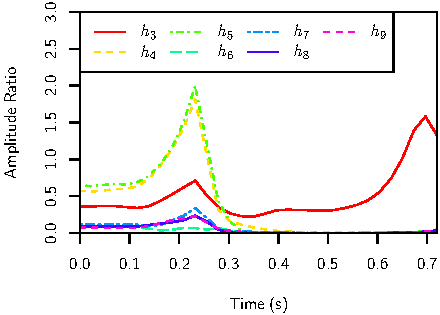
\includegraphics{chapter7/Images/CelloReleaseAmplitudes.pdf}
				\label{fig:CelloRelease}
			}
			\quad
			\subfloat[Clarinet Signal]
			{
				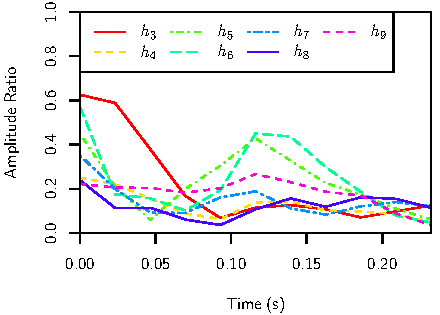
\includegraphics{chapter7/Images/ClarinetReleaseAmplitudes.pdf}
				\label{fig:ClarinetRelease}
			}

			\subfloat[Piano Signal]
			{
				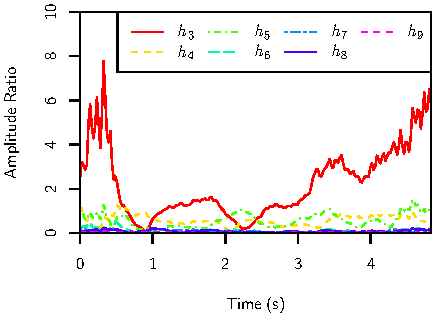
\includegraphics{chapter7/Images/PianoReleaseAmplitudes.pdf}
				\label{fig:PianoRelease}
			}
			\caption{Amplitude ratios between the harmonics and fundamental in the release
				 portions of the test signals.}
			\label{fig:ReleaseAmplitudes}
		\end{figure}

		Figure \ref{fig:ReleaseAmplitudes} shows the amplitude ratios between the harmonics and fundamental for the
		release portions of the test signals. The synthesised signal is not included as it has an instantaneous
		release. Both the cello and clarinet signals (Figures \ref{fig:CelloRelease} and \ref{fig:ClarinetRelease})
		exhibit typical envelopes in their release sections, the amplitudes of the higher order harmonics decay
		more quickly than that of the fundamental. In the cello signal however the 3\super{rd} harmonic is the most
		dominant being the last partial in the signal to decay fully. In the piano signal's release section (Figure
		\ref{fig:PianoRelease}) the 3\super{rd} harmonic is again very dominant but the damped fundamental must be
		taken into account when considering the relevance of this.

		The degree to which the relationships between the harmonics' amplitudes in a signal differ from those
		assumed by the reconstruction systems can be measured as the sum of the standard deviations of each of the
		harmonic amplitude ratios. This harmonic variability ($\textrm{HV}$) is measured using Equation
		\ref{eq:HarmonicVariability}. 		
		
		\begin{gather}
			\mu_{n} = \frac{\sum_{f = 1}^{F} \frac{h_{n,f}}{h_{1,f}}}{F} \nonumber \\
			\sigma_{n} = \sqrt{\frac{\sum_{f = 1}^{F} 
					         \left(\frac{h_{n,f}}{h_{1,f}} - \mu_{n} \right)^{2}}{F}} \nonumber \\
			\textrm{HV} = \sum_{n = 3}^{9} \sigma_{n}
			\label{eq:HarmonicVariability}
		\end{gather}

		Where $h_{n,f}$ is the amplitude of the $n$\super{th} harmonic in the $f$\super{th} frame of the STFT of
		the signal and $F$ the total number of frames in the STFT. Harmonic variability values for the four test
		signals used in this experiment are shown in Table \ref{tab:HarmonicVariabilities}.

		\begin{table}[h!]
			\centering
			\begin{tabular}{|c|c|}
	\hline
	\bf{Signal} & $\textbf{\mathrm{HV}}$ \tabularnewline
	\hline
	\hline
	Cello & 1.19 \tabularnewline
	\hline
	Clarinet & 1.17 \tabularnewline
	\hline
	Synthesised & 1.07 \tabularnewline
	\hline
	Piano & 2.80 \tabularnewline
	\hline
\end{tabular}

			\caption{The harmonic variabilities of the test signals.}
			\label{tab:HarmonicVariabilities}
		\end{table}

		The harmonic variability values provide a measure of how well the reconstruction systems should be able to
		reproduce the test signals. A higher harmonic variability describes a signal which will be less
		convincingly reconstructed. This is confirmed by measuring the correlation between the harmonic variability
		values and the mean scores given to stimuli reconstructed using a particular set of parameters in the
		multiple stimulus test. Correlation values for each of the reconstruction systems and parameter setting
		combinations are given in Table \ref{tab:HarmonicVariabilityCorrelations}. The stimulus numbers refer to
		the different reconstruction systems as in Figures \ref{fig:SMCRNonlin} and \ref{fig:SMCResults}.

		\begin{table}[h!]
			\centering
			\begin{tabular}{|c|c|c|}
	\hline
	\bf{Stimulus} & $\boldsymbol{r}$ & $\boldsymbol{p}$ \tabularnewline
	\hline
	\hline
	2 & -0.757 & 0.243 \tabularnewline
	\hline
	3 & -0.994 & 0.006 \tabularnewline
	\hline
	4 & -0.998 & 0.002 \tabularnewline
	\hline
\end{tabular}
\qquad
\begin{tabular}{|c|c|c|}
	\hline
	\bf{Stimulus} & $\boldsymbol{r}$ & $\boldsymbol{p}$ \tabularnewline
	\hline
	\hline
	5 & -0.926 & 0.074 \tabularnewline
	\hline
	6 & -0.997 & 0.003 \tabularnewline
	\hline
	7 & -0.999 & 0.001 \tabularnewline
	\hline
\end{tabular}
\qquad
\begin{tabular}{|c|c|c|}
	\hline
	\bf{Stimulus} & $\boldsymbol{r}$ & $\boldsymbol{p}$ \tabularnewline
	\hline
	\hline
	8 & -0.929 & 0.071 \tabularnewline
	\hline
	9 & -0.905 & 0.095 \tabularnewline
	\hline
	10 & -0.978 & 0.022 \tabularnewline
	\hline
\end{tabular}

			\caption{Correlations between the harmonic variabilities of the test signals and 
				 the mean grades given in the multiple stimulus test.}
			\label{tab:HarmonicVariabilityCorrelations}
		\end{table}

		These correlation values suggest that, for all but one of the reconstruction methods, the differences in
		the reconstruction quality between the test signals is due to the different relationships between their
		harmonics' amplitudes. For signals reconstructed using the synthesis method with a window length of 50
		samples (stimulus 2) the correlation between scores and harmonic variability is not so definitive. Another
		factor of the signals or system must influence the inaccuracies introduced when reconstructing in this
		manner. Inspecting the amplitude ratios of the harmonics in the reconstructed signals provides a possible
		explanation for this. The amplitudes ratios of the harmonics for the clarinet signal reconstructed using
		the synthesis technique are shown in Figure \ref{fig:STFTModulations}.

		\begin{figure}[h!]
			\centering
			\captionsetup[subfigure]{oneside,margin={1cm, 0cm}}
			\subfloat[50 Sample Window Length]
			{
				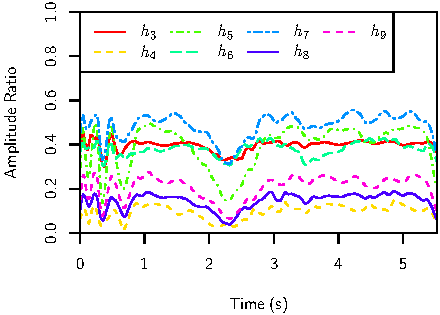
\includegraphics{chapter7/Images/ClarinetSTFT50SustainAmplitudes.pdf}
				\label{fig:ClarinetSTFT50Sustain}
			}
			\quad
			\subfloat[100 Sample Window Length]
			{
				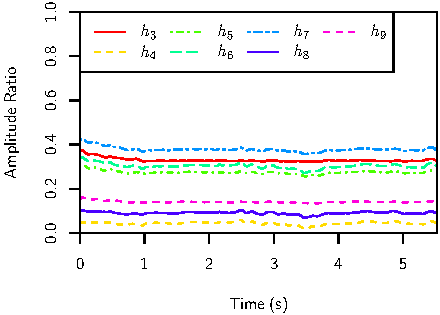
\includegraphics{chapter7/Images/ClarinetSTFT100SustainAmplitudes.pdf}
				\label{fig:ClarinetSTFT100Sustain}
			}

			\subfloat[500 Sample Window Length]
			{
				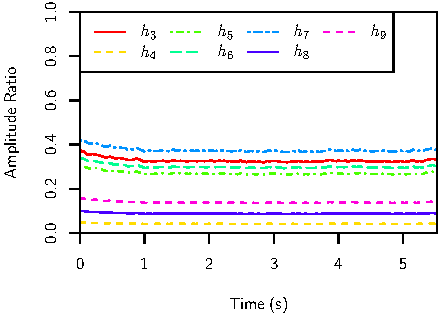
\includegraphics{chapter7/Images/ClarinetSTFT500SustainAmplitudes.pdf}
				\label{fig:ClarinetSTFT500Sustain}
			}
			\caption{Amplitude ratios between the harmonics and fundamental in the sustain portion
				 of the clarinet signal reconstructed with the synthesis technique.}
			\label{fig:STFTModulations}
		\end{figure}

		A window length of 50 samples does not provide the synthesis reconstruction system with enough spectral
		resolution to accurately track the amplitude envelope of the fundamental. As a result the generated
		harmonics do not have a consistent amplitude relationship with the fundamental as seen in Figure
		\ref{fig:ClarinetSTFT50Sustain}. Figures \ref{fig:ClarinetSTFT100Sustain} and
		\ref{fig:ClarinetSTFT500Sustain} show that longer window lenghts allow the amplitude envelope of the
		fundamental to be tracked more accuratly, meaning the generated harmonics follow its amplitude envelope
		move consistently.
		
	\subsection{Conclusion}
	\label{sec:PerceptualExperiments-Reconstruction-Conclusion}
		It has been shown that the `naturalness' of harmonics generated using the information present in the
		fundamental of a signal depends on both the method of generating the harmonic and the properties of the
		input signal. If sufficient processing is applied (increasing the STFT window length / filter order) all
		three of the tested harmonic generation methods perform similarly well. As the amount of processing is
		decreased (decreasing STRT window length / filter order) the synthesis method's performance decreases more
		rapidly than that of the SSBA and IAP based systems. For a given reconstruction system the amplitude
		envelopes of the harmonics in the input signal determine how easily it can be reconstructed. Signals in
		which the harmonics have amplitude envelopes which are linearly related to that of the fundamental are
		reconstructed with better quality than those with more complex relationships.
		
		The SSBA and IAP techniques also have the advantage of having lower computational complexity and introduce
		less latency. The synthesis method requires the calculation of the DFT and introduces latency equal to the
		window length used. Of the three tested methods IAP is the most suitable for use the harmonic excitation
		systems due to it being a homogeneous process. As discussed in Section
		\ref{sec:ExcitationEvaluation-Comparison-Homogeneity} this allows it to be applied to a wider range of
		signals with more predictable results.

\section{Semantic Control}
\label{sec:PerceptualExperiments-SemanticControl}
	In this section the findings of Chapter \ref{chap:TimbreEvaluation} are combined with the techniques discussed in
	Chapter \ref{chap:FeatureControl} to develop audio effects with control parameters which relate to specific
	descriptive terms. Two such effects are developed, each with a single `semantic' control parameter which changes
	processing parameters based on three related semantic terms. The performance of these effects is evaluated both
	objectively, by comparison the results discussed in Section \ref{sec:TimbreEvaluation-Analysis-TimbreSpaces}, and
	subjectively in a series of listening tests.

	\subsection{Effect Design}
	\label{sec:PerceptualExperiments-SemanticControl-EffectDesign}
		In this section the design of two harmonic excitation effects with control parameters intended to alter the
		timbre of sounds between two of the descriptor groups identified in Chapter \ref{chap:TimbreEvaluation} is
		discussed. Across both the distortion and equaliser the thee descriptors with the highest agreements scores
		were `warm', `bright' and `crunch'. As such the two effects were designed taking into account the timbral
		groups these descriptors belong to. The first effect, the warmth / harshness effect, is intended to alter
		timbre between the warmth and brightness groups, introducing `warmth' for low parameter values and
		`brightness' for higher parameter values. As `harsh' was shown to be a in the same timbral group as
		`bright' but being a more exaggerated version of it the highest parameter values should introduce
		`harshness'. The second effect, the harshness / crunchiness effect, is intended to alter timbre between the
		between `brightness' and `crunchiness' groups, introducing `crunchiness' for high parameter values and
		`brightness' for lower values. Again, due to `harsh' being a more exaggerated version of `bright' the
		lowest values should produce `harsher' timbres.

		\subsubsection*{Warmth / Harshness}
			The warmth / harshness effect controls the spectral centroid of a signal using a refined version of
			the system given in Figure \ref{fig:TwoBandSpectralCentroidSystem}. Two spectral bands are
			generated, one with a spectral centroid lower than the input signal and one with a higher spectral
			centroid than the input signal. The relative levels of these bands is then adjusted in order to
			adjust the output's spectral centroid. The full system is shown in Figure \ref{fig:WarmHarsh}.

			\begin{figure}[h!]
				\centering
				\begin{tikzpicture}
					\node (In) at (-1, -3.25) {$x[n]$};
					\coordinate (InMid) at (0, -3.25);
					\draw (In) -- (InMid);

					\coordinate (Side1) at (0, -1.25);
					\coordinate (Side2) at (0, -2.25);
					\draw (InMid) -- (Side2);
					\draw (Side2) -- (Side1);

					\node (F0) [draw] at (2, -1.25) {$f_{0}$ Tracker};
					\node (F0Filter) [draw] at (2, -2.25) {LPF};
					\draw (Side2) -- (F0Filter);
					\draw (F0) -- (F0Filter);
					\draw (Side1) -- (F0);

					\node (Centroid) [draw] at (2, -3.25) {$\mu_{s}$ Tracker};
					\draw (InMid) -- (Centroid);

					\node (Add) [operator] at (10.5, -3.25) {+};

					% NLD
					\node (NLD) [draw] at (4.5, -2.25) {Full Wave Rectifier};
					\draw (F0Filter) -- (NLD);

					\node (NLDFilter) [draw] at (7, -2.25) {HPF};
					\draw (NLD) -- (NLDFilter);

					\node (NLDGain) [gain, minimum size=1.7cm] at (8.5, -2.25) {$m_{H}$};
					\draw (NLDFilter) -- (NLDGain);
					\coordinate (NLDOut) at (9.5, -2.25);
					\draw (NLDGain) -- (NLDOut);
					\draw (NLDOut) -- (Add);

					\coordinate (NLDSide) at (7, -3.25);
					\draw (Centroid) -- (NLDSide);
					\draw (NLDSide) -- (NLDFilter);

					% through
					\coordinate (Through) at (0, -4.25);
					\node (ThroughFilter) [draw] at (2, -4.25) {LPF};
					\draw (Through) -- (ThroughFilter);
					\draw (Side2) -- (Through);
					\draw (Centroid) -- (ThroughFilter);
					\node (ThroughGain) [gain, minimum size=1.7cm] at (8.5, -4.25) {$m_{L}$};
					\coordinate (ThroughOut) at (9.5, -4.25);
					\draw (ThroughFilter) -- (ThroughGain);
					\draw (ThroughGain) -- (ThroughOut);
					\draw (ThroughOut) -- (Add);

					\node (Out) at (11.75, -3.25) {$y[n]$};
					\draw (Add) -- (Out);
				\end{tikzpicture}
				\caption{The system employed in the warmth / harshness effect.}
				\label{fig:WarmHarsh}
			\end{figure}

			The low frequency band is generated by low pass filtering the input signal at its spectral
			centroid.  The high frequency band is generated by applying full wave rectification to the isolated
			fundamental of the input signal and high pass filtering at the input's spectral centroid.
			Separating the bands at the spectral centroid in this way ensures that their respective spectral
			centroids sit either side of the input's. Full wave rectification is used to ensure the system is
			homogeneous.

			The parameter of the effect controls the relative gains applied to each of the spectral bands. The
			parameter value, $p$, ranges from 0 to 1 and is used to calculate the gains, $m_{L}$ and $m_{H}$,
			applied to the low and high frequency bands using Equation \ref{eq:WarmHarshParam}.

			\begin{gather}
				m_{L} = p^{3} \nonumber \\
				m_{H} = 1 - m_{L}
				\label{eq:WarmHarshParam}
			\end{gather}

			When $p = 0$  the output is a low pass filtered version of the input signal resulting in a lower
			spectral centroid than the input. This corresponds to transforms  described as `warm' in the SAFE
			dataset. When $p = 1$ the output signal consists primarily of high order harmonics resulting in an
			increase in spectral centroid and corresponding to transforms labelled `harsh' in the SAFE dataset.
			The power to which $p$ is raised was determined experimentally such that when $p = 0.5$ the effect
			applies processing which corresponds to that described as `bright' in the SAFE dataset. 

		\subsubsection*{Harshness / Crunchiness}
			In Chapter \ref{chap:TimbreEvaluation} it was suggested that `crunchiness' is associated with a
			small increase in spectral irregularity and an output signal with a low spectral kurtosis and
			spectral skewness. To attempt to recreate this the harshness / crunchiness effect controls the
			spectral irregularity of a signal along with the proportion of high frequency energy introduced.
			The system is based on that described in Figure \ref{fig:SpectralShapingSystem}. The full system is
			shown in Figure \ref{fig:HarshCrunch}.

			\begin{figure}[h!]
				\centering
				\begin{tikzpicture}
					\node (In) at (-1, -1.85) {$x[n]$};
					\coordinate (InMid) at (0, -1.85);
					\draw (In) -- (InMid);

					\coordinate (Side) at (0, -0.85);
					\draw (InMid) -- (Side);

					\node (F0) [draw] at (2, -0.85) {$f_{0}$ Tracker};
					\node (F0Filter) [draw] at (2, -1.85) {LPF};
					\draw (InMid) -- (F0Filter);
					\draw (F0) -- (F0Filter);
					\draw (Side) -- (F0);

					\node (Add) [operator] at (12.5, -1.85) {+};

					\coordinate (ExciterIn) at (4, -1.85);
					\draw (F0Filter) -- (ExciterIn);

					% the fundamental
					\coordinate (F0In) at (4, 1);
					\node (F0Gain) [gain, minimum size=1.7cm] at (10, 1) {$m_{1}$};
					\draw (F0In) -- (F0Gain);
					\coordinate (F0Out) at (11, 1);
					\draw (F0Gain) -- (F0Out);
					\draw (F0Out) -- (Add);

					% second harmonic
					\coordinate (F1In) at (4, -0.7);
					\draw (F0In) -- (F1In);
					\node (F1) [draw] at (6, -0.7) {2\super{nd} Harmonic};
					\draw (F1In) -- (F1);

					\node (F1Filter) [draw] at (8.5, -0.7) {BPF};
					\draw (F1) -- (F1Filter);

					\node (F1Gain) [gain, minimum size=1.7cm] at (10, -0.7) {$m_{2}$};
					\draw (F1Filter) -- (F1Gain);
					\coordinate (F1Out) at (11, -0.7);
					\draw (F1Gain) -- (F1Out);
					\draw (F1Out) -- (Add);

					% sixth harmonic
					\coordinate (F5In) at (4, -3);
					\draw (F1In) -- (F5In);
					\node (F5) [draw] at (6, -3) {6\super{th} Harmonic};
					\draw (F5In) -- (F5);

					\node (F5Filter) [draw] at (8.5, -3) {BPF};
					\draw (F5) -- (F5Filter);

					\node (F5Gain) [gain, minimum size=1.7cm] at (10, -3) {$m_{6}$};
					\draw (F5Filter) -- (F5Gain);
					\coordinate (F5Out) at (11, -3);
					\draw (F5Gain) -- (F5Out);
					\draw (F5Out) -- (Add);

					\draw [dots] (F1) -- (F5);
					\draw [dots] (F1Filter) -- (F5Filter);
					\draw [dots] (F1Gain) -- (F5Gain);

					% high order harmonics
					\coordinate (HighIn) at (4, -4.7);
					\draw (F5In) -- (HighIn);
					\node (High) [draw] at (6, -4.7) {Full Wave Rectifier};
					\draw (HighIn) -- (High);

					\node (HighFilter) [draw] at (8.5, -4.7) {HPF};
					\draw (High) -- (HighFilter);

					\node (HighGain) [gain, minimum size=1.7cm] at (10, -4.7) {$m_{H}$};
					\draw (HighFilter) -- (HighGain);
					\coordinate (HighOut) at (11, -4.7);
					\draw (HighGain) -- (HighOut);
					\draw (HighOut) -- (Add);

					\node (Out) at (13.75, -1.85) {$y[n]$};
					\draw (Add) -- (Out);
				\end{tikzpicture}
				\caption{The system employed in the harshness / crunchiness effect.}
				\label{fig:HarshCrunch}
			\end{figure}

			Each of the individual harmonics are generated using the IAP technique discussed in Section
			\ref{sec:Excitation-Methods-IAP}. This method was chosen due to it performing the best in the
			experiments in Section \ref{sec:PerceptualExperiments-Reconstruction}. To reduce computational load
			the filter used to isolate the fundamental in this system is a second order IIR low pass filter.
			The use of a low order filter means that there is a higher proportion of high frequency energy
			which remains in the isolated fundamental. This in turn produces more intermodulation components in
			the generated harmonics. Each of the generated harmonics is band pass filtered in order to reduce
			the influence of these intermodulation components. For higher order harmonics this band pass
			filtering is not effective so only the first six harmonics are generated individually. Again a high
			frequency spectral band is generated by full wave rectifying the isolated fundamental. This high
			frequency band is high pass filtered at the frequency of the sixth harmonic so as not to interfere
			with the individually generated harmonics.

			The effect has one control parameter which ranges from 0 to 1 and controls the relative amplitudes
			of regions of the output spectrum. The spectral irregularity is controlled by adjusting the
			relative levels of the first six harmonics. The analysis and resynthesis technique discussed in
			Section \ref{sec:FeatureControl-Parameterisation-Irregularity} proved to complex to run accurately
			in real time. In its place a simpler system based on a predefined set of harmonic amplitudes,
			$c$, was used. The relative amplitudes of the harmonics are altered as the parameter value, $p$,
			is changed according to Equation \ref{eq:HarshCrunchAmps}.

			\begin{equation}
				a_{n} = p(c_{n} - 1) + 1
				\label{eq:HarshCrunchAmps}
			\end{equation}

			When $p = 0$ the first six harmonics all have the same amplitude, giving the lowest spectral
			irregularity. When $p = 1$ the relative amplitudes of the fort six harmonics are as defined by $c$.
			The values in $c$ are taken from a guitar signal, which had been processed by the SAFE distortion,
			with a Krimphoff irregularity similar to the processed signals in the SAFE dataset described as
			`crunchy'. As the parameter value is increased the spectral irregularity of the first six harmonics
			increases towards that of a `crunchy' signal. This models the increases in spectral irregularity
			noted for the transforms labelled `crunchy' in Chapter \ref{chap:TimbreEvaluation}.
			
			The relative amount of high frequency content in the output is also controlled by $p$. This is
			achieved by changing the relative levels of the band containing the first six harmonics and the
			band generated by the full wave rectifier. The final gains applied to the six generated harmonics
			along with that applied to the rectifier output are given by Equation \ref{eq:HarshCrunchParam}.

			\begin{gather}
				m_{n} = a_{n}\frac{3p + 2}{4} \nonumber \\
				m_{H} = \frac{8 - 7p}{5}
				\label{eq:HarshCrunchParam}
			\end{gather}

			The constants used here were derived experimentally such that when $p = 1$ the amount of energy in
			the high and low bands of the spectrum are roughly equal for a range of input signals. This
			produces the low spectral kurtosis and spectral skewness noticed in signals labeled `crunchy' in
			the SAFE dataset. Lower values of $p$ increase the levels of high frequency energy in the output
			signal causing the spectral transformations associated with `bright' and then `harsh' signals.

	\subsection{Methodology}
	\label{sec:PerceptualExperiments-SemanticControl-Methodology}
		The performance of each effect is evaluated using a set of ten test signals, comprising two electric bass
		guitars (B1 and B2), a flute (F), two electric guitars (G1 and G2), a marimba (M), an oboe (O), a saxophone
		(S), a trumpet (T) and a violin (V). The signals were adjusted to have equal loudness prior to
		experimentation.  Firstly the effects are evaluated objectively by comparing them to the analysis performed
		in Chapter \ref{chap:TimbreEvaluation}. Secondly the effects are evaluated subjectively in a series of
		perceptual listening tests.

		\subsubsection*{Objective Evaluation}
			The performance of each effect is evaluated objectively by examining how they manipulate the
			features of the test signals. Each effect is used to process each of the test signals with its
			parameter set to the minimum value, the middle value and the maximum value, corresponding to
			`warm', `bright' and `harsh' for the warmth / harshness effect and `harsh', `bright' and `crunchy'
			for the harshness / crunchiness effect. The audio features of the unprocessed and processed signals
			in each of these applications are calculated in the same manner as in the SAFE plug-ins. These
			audio features are the compared to those taken from the SAFE dataset.

			As discussed in Chapter \ref{chap:TimbreEvaluation} the terms `warm', `harsh' and `bright' are all
			used to describe transformations applied by both distortion and equalisation effects. `Harsh' and
			`bright' having different definitions depending on the type of processing applied. The objective
			performance of the effects proposed in this section is evaluated against data from both the SAFE
			distortion and equaliser. In order to do this, two new timbre spaces are constructed by performing
			PCA on the processed audio features and feature differences of the combined distortion and
			equaliser data. Two performance scores are given to each combination of audio effect, descriptor
			and test signal. The first measuring how close the processed features of the signal are to points
			labelled with the descriptor in the processed feature timbre space.  The second measuring how close
			the changes in features caused by the effect are to points labelled with the descriptor in the
			feature difference timbre space.

			The performance of a particular effect, with a particular parameter setting on a particular test
			signal is measured by projecting the extracted audio features to a point on the relevant timbre
			space. The processed features of the signal are projected onto the processed feature timbre space
			and the feature differences onto the feature difference timbre space. The Mahalanobis distance,
			$M(x, d)$, between this point, $x$, and the distribution of transforms labelled with the
			descriptor, $d$, is taken using Equation \ref{eq:Mahalanobis}
			
			\begin{equation}
				M(x, d) = \sqrt{(x - \mu_{d})^{T}\Sigma_{d}^{-1}(x - \mu_{d})}
				\label{eq:Mahalanobis}
			\end{equation}

			Where $x$ is a column vector containing the coordinates of the point in the timbre space, $\mu_{d}$
			a column vector containing the mean coordinates of all transforms in the timbre space labelled with
			descriptor $d$ and $\Sigma_{d}$ the covariance matrix of those transforms' coordinates in the
			timbre space. The number of coordinates used in the calculation of Mahalanobis distance is
			determined in the same manner as discussed in Section
			\ref{sec:TimbreEvaluation-Analysis-Agreement}. Where there more than five transforms in the
			distribution, the coordinates in the first five PCs of the timbre space are used. Where the number
			of points in the distribution, $N_{d}$, is lower, only the first $N_{d} - 1$ coordinates can be
			used in order to avoid $\Sigma_{d}$ being singular.

			Where the descriptor, $d$, is represented by two distributions of transforms, one from the
			distortion and one from the equaliser, the Mahalanobis distance from both distributions is taken
			and the minimum distance kept as the measure of performance.
	
		\subsubsection*{Subjective Evaluation}
			To assess the performance of the developed effects subjectively a series of perceptual listening
			tests were undertaken. For the purposes of testing each of the effect was implemented as an audio
			plug-in. Participants were presented with a DAW session containing a track for each of the test
			signals. On each track both effect plug-ins were inserted. The effects were labelled as ``Plug-In
			1'' and ``Plug-In 2'' and had identical interfaces as seen in Figure \ref{fig:TestPlugInterface}.

			\begin{figure}[h!]
				\centering
				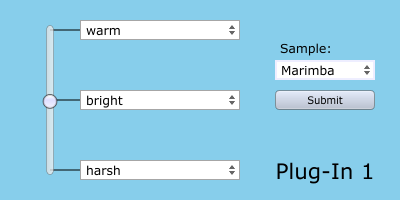
\includegraphics[width=0.6\textwidth]{chapter7/Images/TestPlugInInterface.png}
				\caption{The interface used for assessing the performance of the developed effects.}
				\label{fig:TestPlugInterface}
			\end{figure}

			To mitigate influence of the plug-in's interface layout on the result of the experiment the
			direction of the parameter sliders was randomised for each participant. The order of the tracks in
			the DAW session was also randomised to mitigate any effect the order of tracks may have on results.

			For each effect, on each signal, participants were asked to first take a short time to audition the
			effect to become accustomed to how changing the parameter value affects that particular input
			signal. Once they had investigated the operation of the effect they were asked to label the
			parameter slider at three positions (parameter values of 0, 0.5 and 1) with a term they felt best
			described the timbral effect of the effect at that parameter setting. A list of available terms was
			provided in a drop down list at each parameter value to be labelled as seen in Figure
			\ref{fig:TestPlugInterface}. The available terms were the 17 unique terms from the SAFE dataset
			discussed in Chapter \ref{chap:TimbreEvaluation} (airy, boomy, boxy, bright, clear, creamy,
			crunchy, deep, full, fuzzy, harsh, muddy, raspy, smooth, thin, tinny and warm).

			For each combination of signal, effect and parameter position there is an intended descriptor
			(those the effects were designed to elicit) and a descriptor provided by the participant. The
			relationships between these responses are assessed in two ways. Firstly, participant's responses
			are compared against the clustering performed in Section
			\ref{sec:TimbreEvaluation-Analysis-TermClustering}. The dendrograms shown in Figure
			\ref{fig:CombinedClusters} provide information about how similar the signals / transforms described
			by certain terms are. This information can be used as a metric describing the proximity of the
			user's response to the intended response. The proximity of two descriptors is measured as the
			cophenetic distance between the clusters in which the two descriptors lie. Where a descriptor
			appears twice in the dendrogram (from both the distortion and equaliser) the combination of points
			which yield the lowest cophenetic distance is used. Secondly, heat maps are plotted comparing the
			usage of the 17 available descriptors against the intended descriptors.

			Listening tests were undertaken using circumaural headphones in a quiet listening environment. In
			total 22 participants took part in the listening tests, all of whom reported no know hearing
			problems. On average participants took 25 minutes to complete the test.

	\subsection{Results}
	\label{sec:PerceptualExperiments-SemanticControl-Results}
		\subsubsection{Mahalanobis Distances}
			The Mahalanobis distances between the test signals after being processed by the warmth / harshness
			effect and those in the timbre space constructed from the SAFE dataset are shown in Figure
			\ref{fig:HarshJeffs}. Distances in both the processed feature space and the feature difference
			space are shown in Figures \ref{fig:HarshProcJeff} and \ref{fig:HarshDiffJeff} respectively.

			\begin{figure}[h!]
				\centering
				\captionsetup[subfigure]{oneside,margin={1cm, 0cm}}
				\subfloat[Processed Featues]
				{
					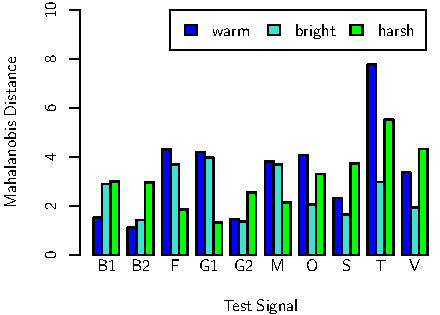
\includegraphics{chapter7/Images/HarshProcessedJeffsDistance.pdf}
					\label{fig:HarshProcJeff}
				}
				\quad
				\subfloat[FeatureDifferences]
				{
					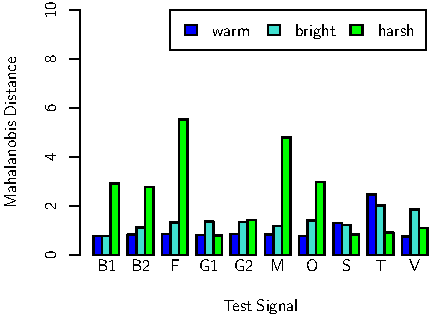
\includegraphics{chapter7/Images/HarshDifferenceJeffsDistance.pdf}
					\label{fig:HarshDiffJeff}
				}
				\caption{Mahalanobis distances for the warmth / harshness effect.}
				\label{fig:HarshJeffs}
			\end{figure}

			The Mahalanobis distances between the test signals after being processed by the harshness /
			crunchiness effect and those in the timbre space constructed from the SAFE dataset are shown in
			Figure \ref{fig:CrunchJeffs} again separated into separate figures for both the processed feature
			space and feature difference space.

			\begin{figure}[h!]
				\centering
				\captionsetup[subfigure]{oneside,margin={1cm, 0cm}}
				\subfloat[Processed Featues]
				{
					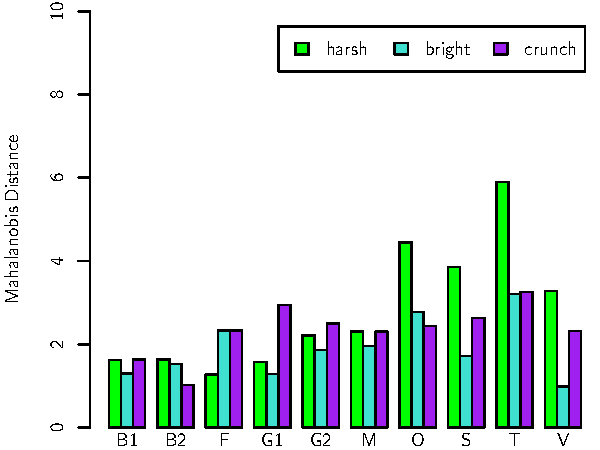
\includegraphics{chapter7/Images/CrunchProcessedJeffsDistance.pdf}
					\label{fig:CrunchProcJeff}
				}
				\quad
				\subfloat[FeatureDifferences]
				{
					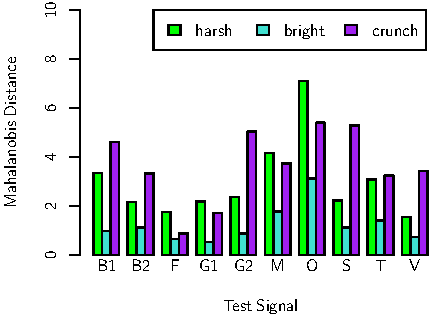
\includegraphics{chapter7/Images/CrunchDifferenceJeffsDistance.pdf}
					\label{fig:CrunchDiffJeff}
				}
				\caption{Mahalanobis distances for the harshness / crunchiness effect.}
				\label{fig:CrunchJeffs}
			\end{figure}

		\subsubsection{Listening Test Results}
			The mean cophenetic distances between participants' annotation of the warmth / harshness effect's
			parameter and the descriptors `warm', `bright' and `harsh' are shown in Figure
			\ref{fig:HarshCophs}, The error bars representing the 95\% confidence interval for each mean.
			Cophenetic distances in both the processed feature dendrogram (Figure
			\ref{fig:CombinedProcessedClusters}) and the feature difference dendrogram (Figure
			\ref{fig:CombinedDifferenceClusters}) are shown in Figures \ref{fig:HarshProcCoph} and
			\ref{fig:HarshDiffCoph} respectively.

			\begin{figure}[h!]
				\centering
				\captionsetup[subfigure]{oneside,margin={1cm, 0cm}}
				\subfloat[Processed Featues]
				{
					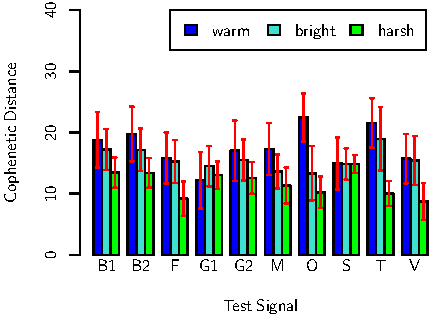
\includegraphics{chapter7/Images/HarshProcessedCophDistance.pdf}
					\label{fig:HarshProcCoph}
				}
				\quad
				\subfloat[FeatureDifferences]
				{
					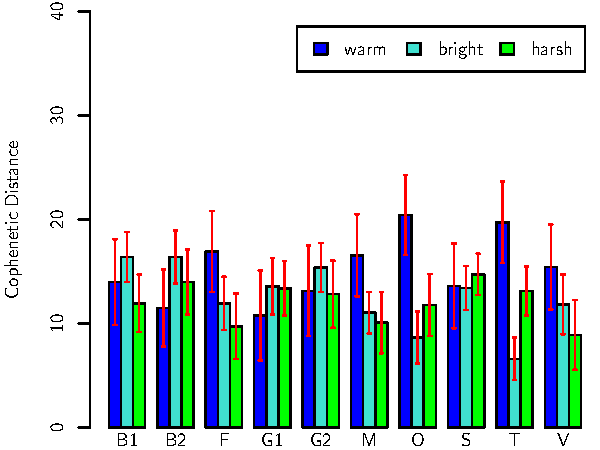
\includegraphics{chapter7/Images/HarshDifferenceCophDistance.pdf}
					\label{fig:HarshDiffCoph}
				}
				\caption{Cophenetic distances for the warmth / harshness effect.}
				\label{fig:HarshCophs}
			\end{figure}

			The mean cophenetic distances between participants' annotation of the harshness / crunchiness
			effect's parameter and the descriptors `harsh', `bright' and `crunch' are shown in Figure
			\ref{fig:HarshCophs}. Again, distances in both the processed feature dendrogram and
			feature difference dendrogram are shown separately.

			\begin{figure}[h!]
				\centering
				\captionsetup[subfigure]{oneside,margin={1cm, 0cm}}
				\subfloat[Processed Featues]
				{
					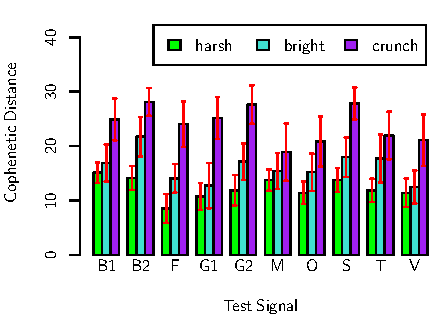
\includegraphics{chapter7/Images/CrunchProcessedCophDistance.pdf}
					\label{fig:CrunchProcCoph}
				}
				\quad
				\subfloat[FeatureDifferences]
				{
					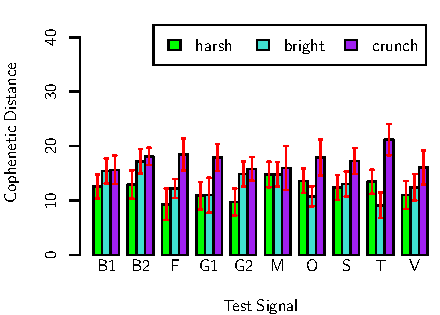
\includegraphics{chapter7/Images/CrunchDifferenceCophDistance.pdf}
					\label{fig:CrunchDiffCoph}
				}
				\caption{Cophenetic distances for the harshness / crunchiness effect.}
				\label{fig:CrunchCophs}
			\end{figure}

			Figures \ref{fig:HarshConfusion}, \ref{fig:CrunchConfusion} and \ref{fig:CombConfusion} show heat
			maps comparing the usage of terms by test participants and the terms the effects were designed to
			control. Figure \ref{fig:HarshConfusion} for the results collected from the warmth / harshness
			effect, Figure \ref{fig:CrunchConfusion} for the harshness / crunchiness effect and
			\ref{fig:CombConfusion} the combination of data from both effects. Each cell in the figures
			represents the frequency with which one of the available descriptors (bottom) was used to describe
			the timbral effect at the parameter position which was intended to produce a particular timbral
			result (right). Above the figure is a dendrogram representing the clustering of terms based on
			their frequency of usage.

			\begin{figure}[h!]
				\centering
				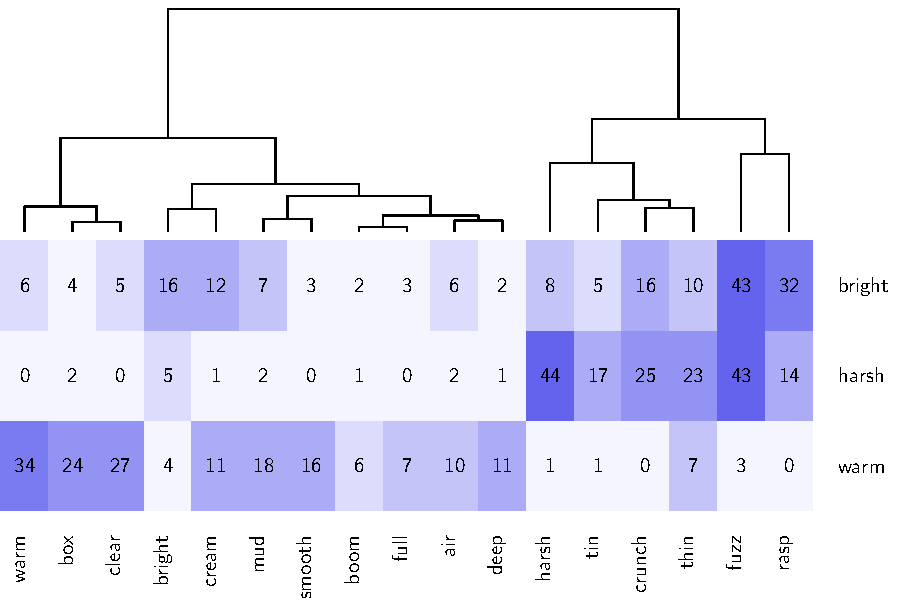
\includegraphics{chapter7/Images/HarshConfusion.pdf}
				\caption{Heat map of term usage for the warmth / harshness effect.}
				\label{fig:HarshConfusion}
			\end{figure}

			\begin{figure}[h!]
				\centering
				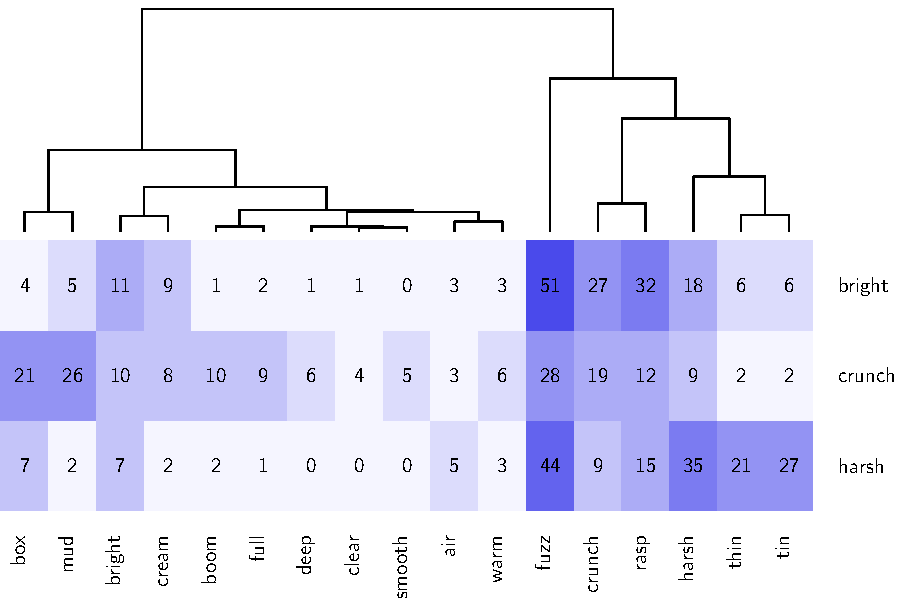
\includegraphics{chapter7/Images/CrunchConfusion.pdf}
				\caption{Heat map of term usage for the harshness / crunchiness effect.}
				\label{fig:CrunchConfusion}
			\end{figure}

			\begin{figure}[h!]
				\centering
				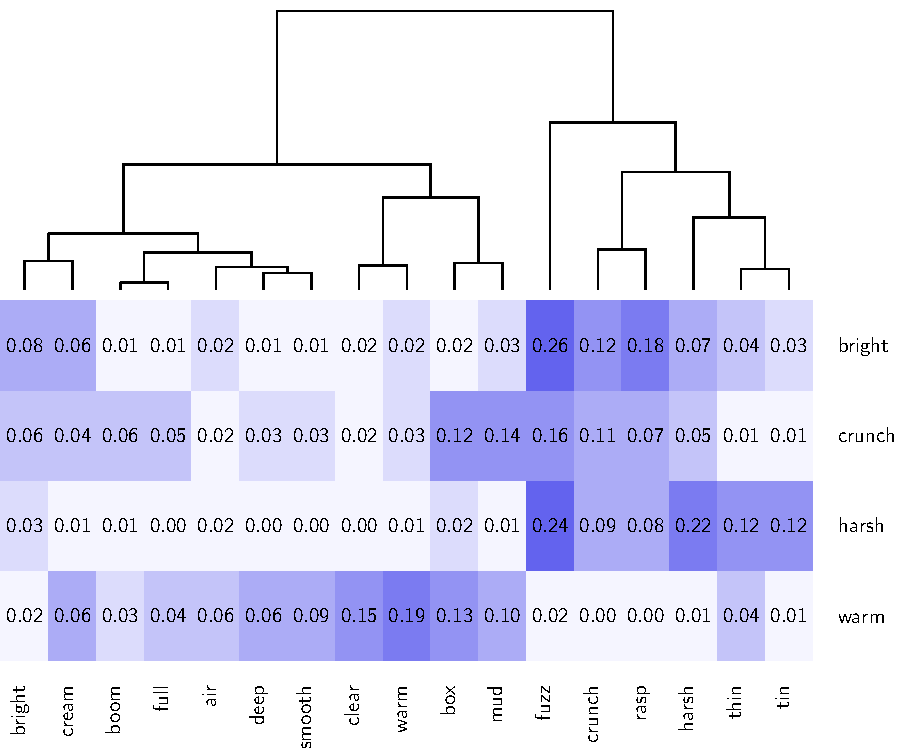
\includegraphics{chapter7/Images/CombinedConfusion.pdf}
				\caption{Heat map of term usage across both effects.}
				\label{fig:CombConfusion}
			\end{figure}

	\subsection{Discussion}
	\label{sec:PerceptualExperiments-SemanticControl-Discussion}
		\subsubsection*{Warmth / Harshness Effect}
			It was determined in Chapter \ref{chap:TimbreEvaluation} that the descriptors `warm', `bright' and
			`harsh' are best defined by relative changes in audio features rather than absolute values of
			features in the output signal. `Warmth' describing transforms which shift spectral energy towards
			lower frequencies and `brightness' and `harshness' describing transforms which introduce increasing
			proportions of high frequency energy. Because of this, distances measured in the processed feature
			space (Figures \ref{fig:HarshProcJeff} and \ref{fig:HarshProcCoph}) do not give as good a measure
			of performance as those in the feature difference space (Figure \ref{fig:HarshDiffJeff} and
			\ref{fig:HarshDiffCoph}).

			The results in Figure \ref{fig:HarshDiffJeff} imply that the warmth / harshness effect is
			successful in applying transforms similar to those described as `warm' and `bright' in the SAFE
			dataset. For the majority of the input signals the Mahalanobis distances for the `warm' and
			`bright' transforms are close to 1, indicating that the transform fits well within the distribution
			of other transforms labeled with these descriptors in the timbre space.
			
			When attempting to make the test signals `harsher' however, the effect does not perform well on the
			bass guitar, flute, marimba or oboe signals. This is likely due to the small number of transforms
			labelled harsh in the timbre space. In Chapter \ref{chap:TimbreEvaluation} `harsh' was given a low
			agreement score in both the distortion and equaliser timbre spaces due to there only being four
			transforms labeled `harsh' in each space. As such, only a small region of the timbre space is
			described as harsh, making it more difficult to design a transform which will sit in that region
			for a wide range of input signals.
			
			Examining the mean cophenetic distances in Figure \ref{fig:HarshDiffCoph} it might appear that
			while listening test participants do not always use the terms which the warmth / harshness effect
			was designed to elicit, on average they use terms which lie in the same cluster. Referring to
			Figure \ref{fig:CombinedDifferenceClusters} we find three main clusters, which could be described
			as `warmth' (containing the terms `mud', `boom', `smooth', `crunch', `full', `deep', `warm' and
			`cream'), `distorted brightness' (containing the terms `fuzz', `bright', `harsh', `box' and `rasp')
			and `equalised brightness' (containing the terms 'clear', `bright', `tin', `thin', `air' and
			`harsh'). These three clusters have heights of 17.3, 13.5 and 16.5 respectively. The mean
			cophenetic for each of the test signals all lie close to or below these cluster heights. Further
			analysis is required to determine whether this indicates that participants are using terms in the
			relevant clusters.

			Figure \ref{fig:HarshConfusion} shows that `warm' was the most commonly used term to describe the
			effect of the warmth / harshness effect when its parameter is set to `warm', followed by `clear',
			`box' and `mud'. These descriptors lie across all three of the clusters identified in Figure
			\ref{fig:CombinedDifferenceClusters}. Summing the cells of this figure it is found that
			participants only used descriptors in the same cluster as `warm' 54\% of the time. The mean
			cophenetic distances for the `warm' transform in Figure \ref{fig:HarshDiffCoph} do not represent
			participants using descriptors from the correct cluster. The failure of the effect to elicit terms
			related to warmth from participants may indicate that warmth is not only defined by a shift in
			spectral energy towards lower frequencies. Examining figure \ref{fig:HarshProcJeff} it is seen
			that, for approximately half the test signals, the processed signals are significantly distant from
			the region described as `warm' in the processed feature space constructed from the SAFE dataset.
			
			Considering only the changes in audio features described by transforms, the terms `bright' and
			`harsh' seem to have different definitions depending on the type of processing applied, as seen in
			Chapter \ref{chap:TimbreEvaluation}. The results of this listening test, however, suggest that
			these terms may be more closely related. The differences in their clustering being due only to the
			differences in processing rather than differences in perception. Figure \ref{fig:HarshConfusion}
			shows that, when describing the effect of the warmth / harshness effect, participants used a
			descriptor related to the intended descriptor 74\% of the time for `bright' and 80\% of the time
			for `harsh'. The terms used come from both the `distorted brightness' and `equalised brightness'
			clusters, suggesting that although some of these terms were gathered using the SAFE Equaliser they
			can still be applied to distortion type effects. Even so, the most commonly used descriptors,
			`fuzz', `harsh' and `rasp' all lie within the `distorted brightness' cluster. The use of terms
			which were collected from the SAFE equaliser may be explained by the anonymity of the effects in
			this test. While using the SAFE plug-ins the user is aware of the type of effect they are using so
			may be more likely to use descriptors they associate with that effect. In this test the type of
			effect is not know to the user so they may select descriptors they would not usually associate with
			the type of effect being used.

			The listening test data does not represent a difference between `bright' and `harsh' as seen in
			Chapter \ref{chap:TimbreEvaluation}. Both the `bright' and `harsh' positions of the warmth /
			harshness effect's parameter were labelled as `fuzzy' the most often. The `harsh' position was
			labelled as `harsh' more often than the `bright' position, suggesting that the `harsh' position on
			the slider produces `harsher' transforms than the `bright' position, but not that `harsh' does not
			apply as a descriptor to the `bright' position.
			
		\subsubsection*{Harshness / Crunchiness Effect}
			In Chapter \ref{chap:TimbreEvaluation} it was concluded that `crunchiness' is defined by an output
			signal with energy spread evenly throughout the spectrum and a slight increase in spectral
			irregularity. This means that, when attempting to make signals sound `crunchier', both the
			processed features and feature differences are relevant.  Figure \ref{fig:CrunchProcJeff} shows
			that for the majority of the input signals the harshness / crunchiness effect produces output
			signals which are close to those labeled as `crunchy' in the SAFE dataset. However, the transforms
			applied to produce these signals are less similar to those in the SAFE dataset, as seen in Figure
			\ref{fig:CrunchDiffJeff}. This is possibly explained by the simplifications made to reduce the
			effect's computational complexity. Using lower order filters increases the level of intermodulation
			components in the individually generated harmonics. Controlling the relative levels of these
			generated harmonics no longer has the expected effect on spectral irregularity as each generated
			harmonic contains several spectral partials with unknown amplitudes.

			For the harshness / crunchiness effect's `bright' and `harsh' parameter settings only the measures
			of Mahalanobis distance in the feature difference space are relevant (is in the analysis of the
			warmth / harshness effect). In this regard the effect is most accurate in recreating transforms
			labelled `bright' in the SAFE dataset, having similar performance to the warmth / harshness effect.
			For its `harsh' parameter setting it is less accurate, again possibly due to the low confidence
			definition of the term `harsh' due to it being used with very low frequency in the SAFE dataset.

			In Figure \ref{fig:CombinedClusters} the term `crunch' sits in different clusters depending on the
			features used for clustering. When clustering using processed features it sits in a cluster
			alongside `tin', `harsh', `full', `thin', `air' and `clear', whereas using the feature differences
			it is part of the `warmth' cluster described previously. Examining the mean cophenetic distances
			from the listening test (Figure \ref{fig:CrunchCophs}) it appears that participants used terms
			which cluster closer to `crunch' in the feature difference space when labelling the harshness /
			crunchiness effect's `crunch' parameter position. Summing the relevant cells in the heat map shown
			in Figure \ref{fig:CrunchConfusion} is is seen that using the clusters calculated from processed
			features, participants only used terms in the same cluster as `crunch' 17\% of the time. Whereas
			when using the feature difference this figure rises to 51\%. This might suggest that `crunch' is
			better defined by properties of the transform rather than of the output signal.

			The performance of the harshness / crunchiness effect in its `bright' and `harsh' parameter
			settings is similar to that of the warmth / harshness effect. The mean cophenetic distances in the
			feature difference space (Figure \ref{fig: }) are low, suggesting that participants are selecting
			descriptors in the relevant clusters. Referring to the heat map in Figure \ref{fig:CrunchConfusion}
			it is seen that a descriptor from a relevant cluster is used 72\% of the time for the `bright'
			parameter setting and 90\% of the time for the `harsh' parameter setting. Both the warmth /
			harshness and harshness / crunchiness effects behave similarly in their `bright' and `harsh'
			parameter parameter settings, introducing a high pass filtered version of the full wave rectified
			fundamental. Again `fuzz' is the most commonly used descriptor for both parameter settings.

		\subsubsection*{Descriptor Clustering}
			The results of the listening test can be further analysed by clustering terms based on how often
			they were used to describe particular a particular combination of signal, effect and parameter
			setting. This clustering can be used to identify synonyms and compare them with the timbral groups
			identified in Chapter \ref{chap:TimbreEvaluation}. Dendrograms of this clustering are shown on the
			heat maps in Figures \ref{fig:HarshConfusion}, \ref{fig:CrunchConfusion} and
			\ref{fig:CombConfusion}.

			Across all three heat maps the terms group into two main clusters. A `fuzziness' cluster
			(containing terms such as `fuzz', `rasp', `crunch' and `harsh') and a `warmth' cluster (containing
			terms such as `warm', `mud', `full' and `cream'). This can be seen as a lower resolution version of
			the clustering performed in Chapter \ref{chap:TimbreEvaluation} combining the warmth and muddiness
			clusters and the brightness and crunchiness clusters. The two clusters identified represent
			transforms which introduce a larger proportion of high frequency energy and those which introduce a
			larger proportion of lower frequency energy.

	\subsection{Conclusion}
	\label{sec:PerceptualExperiments-SemanticControl-Conclusion}
		Both the warmth / harshness and harshness / brightness effects are successful in producing effect which are
		described as `bright' and `harsh'. `Hash' is confirmed to be a more exaggerated version of `bright'
		describing signals with higher proportions of high frequency content. Due to the nature of the processing
		however, other terms are also used to describe these effects suck as `fuzzy' and `raspy'. These terms were
		associated with the SAFE distortion effect in Chapter \ref{chap:TimbreEvaluation} and so it it expected
		that they may get used to describe a harmonic excitation system.

		\note
		{
			When provided with descriptors to use, people might use descriptors they wouldn't necessarily
			provide themselves to describe a sound. So the distortion and equaliser terms both get used.
			Anonymous effect. People labelling a distortion will use distortion like words, but with an
			anonymous effect all words are open.

			\begin{itemize}
				\item Warmth is difficult to elicit.
				\item Harsh was found to be a more exaggerated version of bright. Although related terms
					are used with describe the distorted nature more often.
				\item Brightness and harshness are both simple to elicit through the introduction of a
					high pass filtered distortion.
			\end{itemize}
		}
		

\section{Conclusion}
\label{sec:PerceptualExperiments-Conclusion}
	\note
	{
		In the end it is all silly.
	}
